\documentclass{tufte-handout}
%------------------------------------------------
%\geometry{showframe} % display margins for debugging page layout
%------------------------------------------------
\usepackage{graphicx} % allow embedded images
  \setkeys{Gin}{width=\linewidth,totalheight=\textheight,keepaspectratio}
  \graphicspath{{/home/swl/Dropbox/ucd/eu_economics/figs/}}  % set of paths to search for images
\usepackage{amsmath}  % extended mathematics
\usepackage{booktabs} % book-quality tables
\usepackage{units}    % non-stacked fractions and better unit spacing
\usepackage{multicol} % multiple column layout facilities
\usepackage{lipsum}   % filler text
\usepackage{fancyvrb} % extended verbatim environments
  \fvset{fontsize=\normalsize}% default font size for fancy-verbatim environments

%------------------------------------------------
% Standardize command font styles and environments
\newcommand{\doccmd}[1]{\texttt{\textbackslash#1}}% command name -- adds backslash automatically
\newcommand{\docopt}[1]{\ensuremath{\langle}\textrm{\textit{#1}}\ensuremath{\rangle}}% optional command argument
\newcommand{\docarg}[1]{\textrm{\textit{#1}}}% (required) command argument
\newcommand{\docenv}[1]{\textsf{#1}}% environment name
\newcommand{\docpkg}[1]{\texttt{#1}}% package name
\newcommand{\doccls}[1]{\texttt{#1}}% document class name
\newcommand{\docclsopt}[1]{\texttt{#1}}% document class option name
\newenvironment{docspec}{\begin{quote}\noindent}{\end{quote}}% command specification environment
%------------------------------------------------
\graphicspath{{/home/swl/Dropbox/ucd/eu_economics/figs/}} 

%------------------------------------------------
%%%% Details %%%%
%------------------------------------------------
\title{European Economy: is the EU an optimum currency area?}
\author{University College Dublin}
\date{Spring 2017} 

\begin{document}
\maketitle  
%------------------------------------------------------------------------------
\section{OCA criteria and the EU}
Having discussed optimum currency area theory in the previous lecture, here we will apply the criteria to the European Union to analyse whether it qualifies as an OCA.
Some economists were skeptic about the introduction of a single currency on the grounds that the European countries did not fulfill the economic requirements. 
Ultimately the launch of the Euro was mainly based on political considerations.\footnote{OCA theory was not used in developing the Euro.}
We will discuss criteria set out by Mundell, McKinnon, and Kenen which included
\begin{enumerate}
  \item Labour mobility
  \item Diversification
  \item Openness
  \item Homogeneous preferences
  \item Transfers
  \item Common destiny
\end{enumerate}

%------------------------------------------------------------------------------
\subsection{Labour mobility}
Migration can be an important mitigation strategy in order to deal with asymmetric shocks. 
Additionally, individuals can take advantage of differences in earnings across the different countries, moving to a place where they can earn more. 
Concerning moving from one to another country there are of course a number of obstacles that a migrant has to consider. 
These obstacles are both economic and non-economic in nature. 
In terms of purely economic obstacles on has to consider
\begin{itemize}
  \item The cost of moving itself
  \item The risk of becoming unemployed in the destination country
  \item Prospects for the family
  \item Fiscal factors such as social benefits and taxation on earnings
\end{itemize}
In addition there are non-economic factor that influence the decision to migrate such as
\begin{itemize}
  \item Cultural differences
  \item Links with family and friends
  \item Commitment to origin country
\end{itemize}
Because of these factors labour mobility will always be limited. 
A popular benchmark for European labour mobility is the USA, which has a similar size, level of economic development, and comparable within-area differences.\footnote{Think of Mississippi as a sort of Greece in economic terms.}
Research has shown that European labour mobility is very low compared to the USA.
This applies both to the movement between and within European countries. 
For the EU15 labour mobility
\begin{itemize}
  \item between countries is about a fourth of the US level
  \item within countries is about half of the US level
\end{itemize}

This low level of migration between European countries can be easily explained by some of the factors listed above. 
Concerning the surprisingly low levels of within-country migration, the explanation for this can be found in factors such as the housing market which is not as fluid as in the USA.
The most important implication of low labour mobility across Europe is that when there is an asymmetric shock the likely result will be high levels of unemployment; even in the face of economic adversity people are not willing to look for better opportunities abroad.\footnote{Contrast this with the movement of European to other parts of the world during the 1800s and early part of the 1900s.}

%------------------------------------------------------------------------------
\subsection{Diversification and trade}
Asymmetric shocks can have severe consequences, and given the low levels of labour mobility, lead to high unemployment levels. 
Two of the OCA criteria rest on the idea that the frequency of asymmetric shocks is lower among countries that have 
\begin{itemize}
  \item Similar production patterns
  \item A diversified trade pattern and
  \item are open to trade
\end{itemize}

Although not much research on the topic of product diversification seem to exist, in general most member countries of the European Union have a complex diversified economy and indeed there exist similarities in trade structures across countries.\footnote{R. Horv\'ath (2007). "Ready for Euro? Evidence on EU new member states" Applied Economic Letters (14).}
Although a country such as the Netherlands is dissimilar to the other European countries in terms of trade, possibly due to gas exports, it is still part of the Eurozone. 
This is possibly due to the fact that the Dutch assume the costs outweigh the benefits. 
Other member states such as Poland and Hungary are very similar to the other European countries, but have opted not to adopt the Euro.
Concerning the openness in trade, figure~\ref{fig:trade} shows the sum of exports and imports relative to GDP for 2015 for all EU member states. 
Most European countries are very open to international trade as the figure illustrates.
An interesting pattern here is that many small countries have very high levels of trade.
A country that is heavily involved in international trade, the use of an independent exchange rate is reduced.
%--------------------------------------
\begin{figure}
  \includegraphics[scale=.3]{trade}
  \label{fig:trade}
  \caption{The sum of exports and imports relative to GDP for 2015. Data: World Bank Development Indicators}
\end{figure}
%--------------------------------------

%------------------------------------------------------------------------------
\subsection{Homogeneous preferences}
Moving from the economic to the political criteria, an important criterion is that of homogeneous preferences concerning monetary and fiscal policy.\footnote{Monetary policy is an important tool to deal with macroeconomic shocks. Although some schools of thought within macroeconomics contest this idea.}  
To analyse the degree of similarity in terms of macroeconomic policy across European countries we look at past trends concerning
\begin{itemize}
  \item The inflation rate (for monetary policy)
  \item Public debt (for fiscal policy)
\end{itemize}
Figure~\ref{fig:inflation} shows the inflation rates for Germany, Italy, and Greece over time. 
The figure clearly illustrates that there are some striking differences across countries in terms of preferences with regard to monetary policy.\footnote{The Germans are notoriously squeamish about inflation given their experience with the hyperinflation during the Weimar Republic.} 
Figure~\ref{fig:public_debt} shows the average level of public debt and illustrate that also with regard to fiscal policy there are some alrge differences across countries. 
The fact that the Eurozone is characterised by heterogeneous preferences is something that became painfully clear during the sovereign debt crisis, where in the public debate the fiscal discipline of certain countries was cited as being a main reason to explain the mess which they were in. 

%--------------------------------------
\begin{figure}
  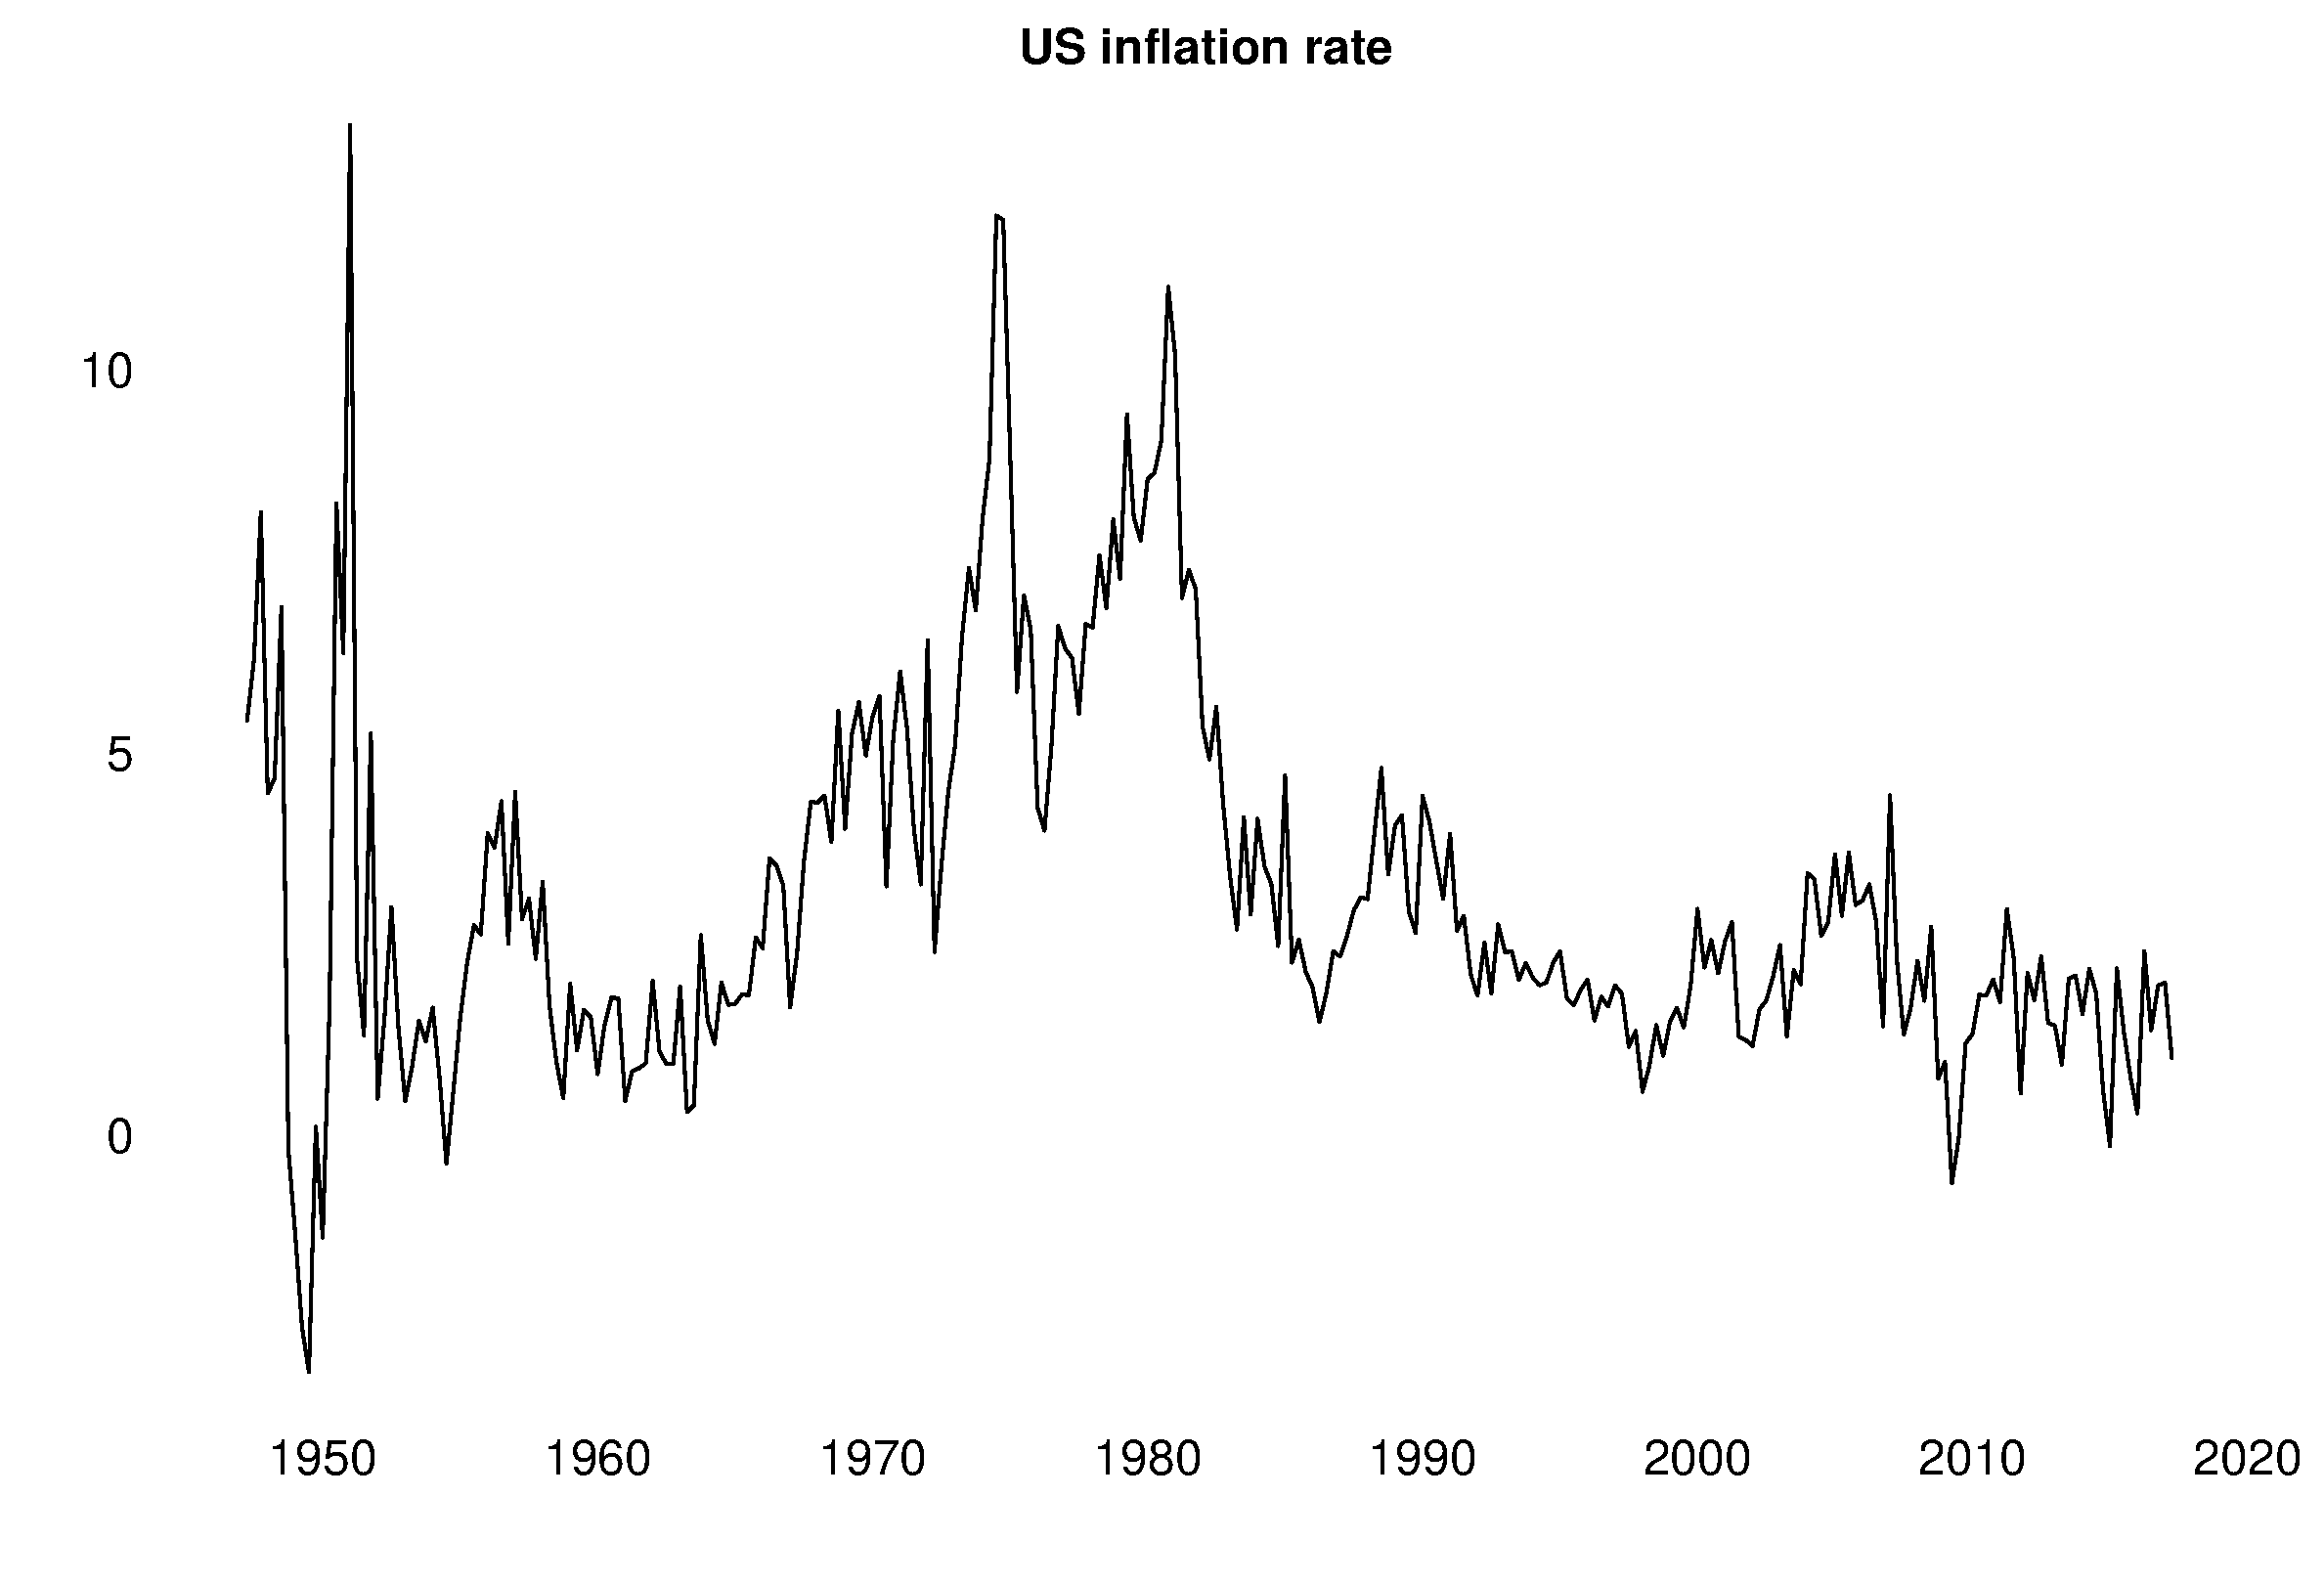
\includegraphics[scale=.3]{inflation}
  \label{fig:inflation}
  \caption{Inflation rate in Germany, Italy, and Greece. Data: Eurostat}
\end{figure}
%--------------------------------------
%--------------------------------------
\begin{figure}
  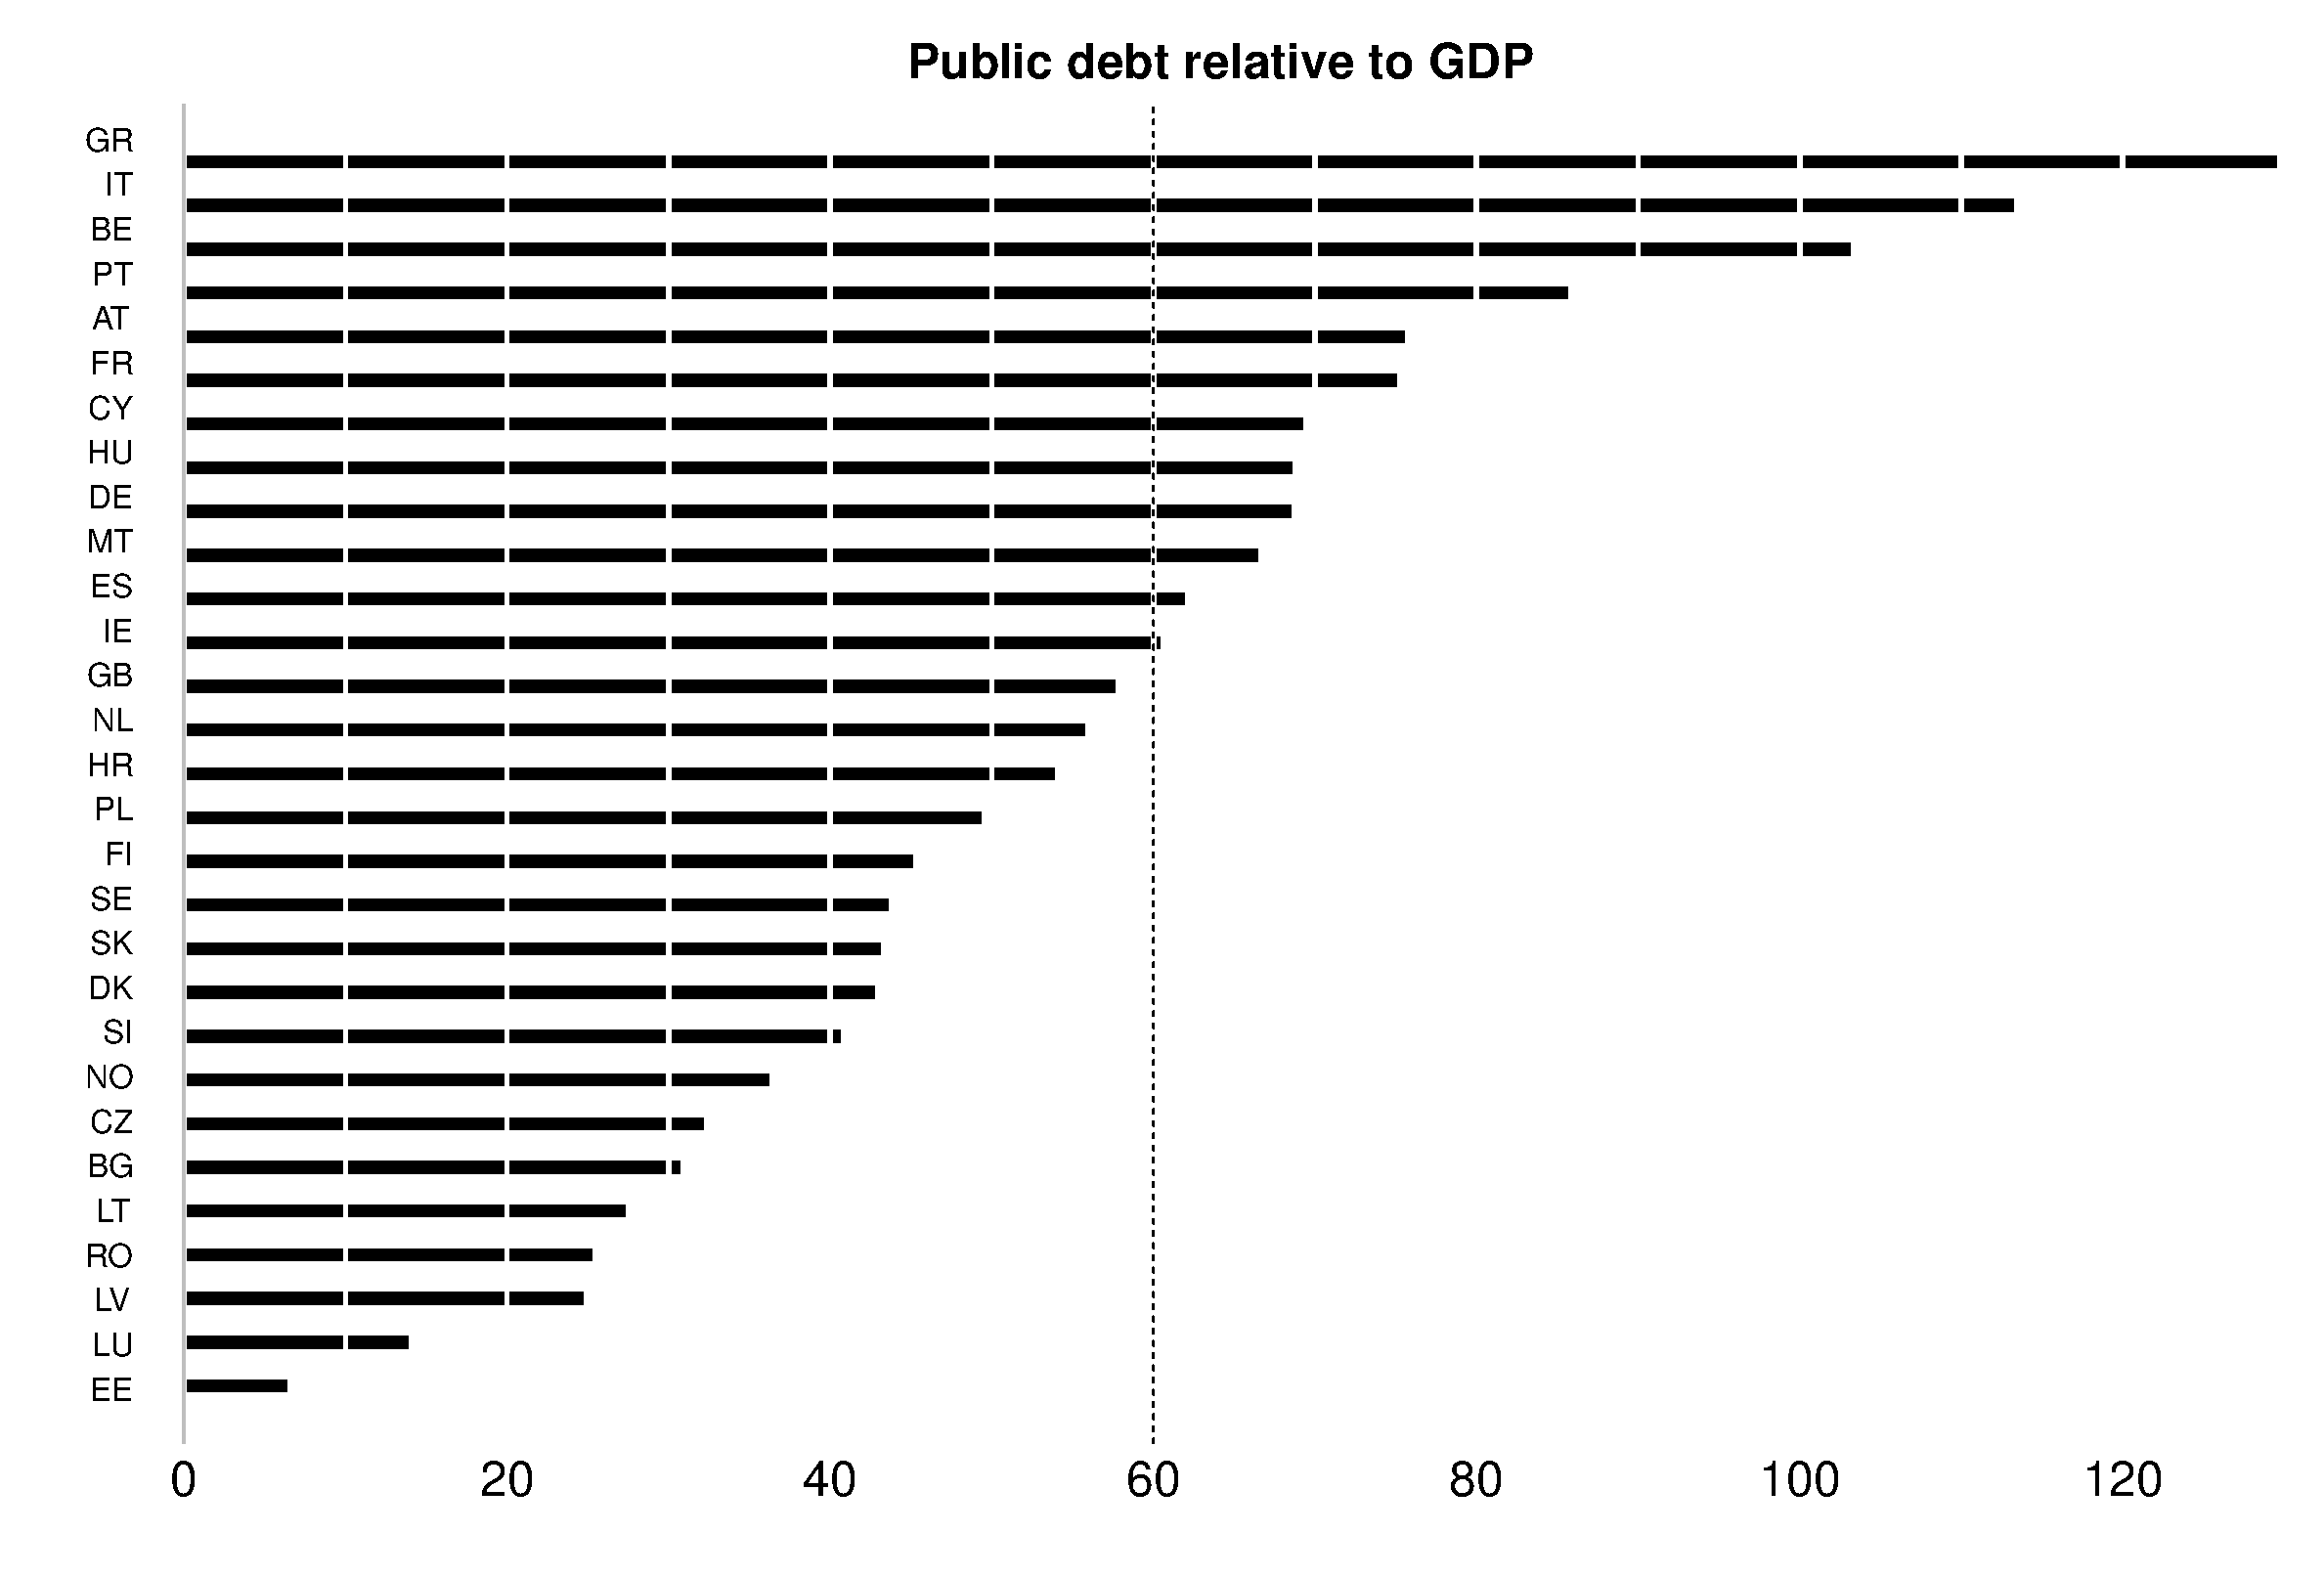
\includegraphics[scale=.3]{public_debt}
  \label{fig:public_debt}
  \caption{Average public debt relative to GDP between 2000-2016. Data: Eurostat}
\end{figure}
%--------------------------------------

\clearpage
Despite the similarities of European countries in terms of regime type, we do see that macroeconomic policies are quite diverse. 
A natural question to ask here is why are there such large differences? 
To answer this question one probably has to look at the incentives that politicians face in their country and which shape their institutions. 
For instance some countries have stronger labour union movements than others, or place more emphasis on public goods provision. 
In order to homogenise preferences across the continent, or the EU member states, one possible step to a solution is to set up common institutions. 
Within the EU a first step towards this has been made with the creation of the European Central Bank (ECB).
The ECB for instance determines the monetary policy for the Eurozone.
The ECB's main objective is to maintain price stability within the Eurozone, which it tries to achieve in cooperation with the national central banks. 
Additionally, in terms of fiscal policy, all the national budgets of EU member states are subject to an excessive debt procedure in order to curtail excessive public spending.\footnote{Both the monetary policy of the ECB and the excessive debt procedure will feature in a future lecture.}
Although certain aspects of macroeconomic stabilitsation are now operated under common institutions does not entail that countries actually agree on the best course of action in dealing with shocks. 
Nonetheless, it is an important step towards tighter monetary integration.

%------------------------------------------------------------------------------
\subsection{Fiscal Transfers}
One of the OCA criteria states that countries should form an OCA when there are fiscal transfers. 
Within the EU and the Eurozone there was no cyclical fiscal transfer system in the EU.
There are a number of programs that transfer money to certain regions, but this is done regardless of whether said region experienced a shock or not. 
In general the budget of the European Union is very small at about only 1\% of the combined GDP of all EU member states. 
This budget is spend mainly on three items
\begin{enumerate}
  \item Structural fund and Cohesion policy (50\%)
  \item Common Agricultural Policy (43\%)
  \item Operating expenses (6\%)
\end{enumerate}
As you might recall, the Structural Fund and the transfer in context of the Cohesion policy are there to help EU regions with a GDP below 75\% of the EU average. 
These are funds to assist with for instance building infrastructure which stimulates the local economy on the long term. 
These funds are transferred for a period of seven years and not cyclical and regardless of whether a region experienced a shock.
For a few years ago there were no provisions concerning fiscal transfer following shocks. 
This changed when the sovereign debt crisis hit a couple of Eurozone countries pretty hard, even increasing the risk of a default. 
In a reaction, albeit slow one, a number of provisions were established in order to provide financial aid such as for instance the European Stability Mechanism (ESM).\footnote{The ESM only includes the Eurozone member states.} 
ESM member states can apply for an ESM bailout when they are in serious financial difficulty or when their banks need recapitalisation. 
The establishment of the ESM was an important first step towards a system of fiscal transfers. 
However, to improve the stability of the Euro a more formalised program is likely required.

%------------------------------------------------------------------------------
\subsection{Europeanism vs. nationalism}
Arguably the hardest criteria to achieve is to create a sense of pan-European solidarity. 
Figure~\ref{fig:public_opinion} shows the results of a Eurobarometer survey from 2006 asking how often people thought of themselves as being European. 
As the figure illustrates there does not seem to be a great sense of Europeanism across countries. 
This is also something that has become clear over the years with the rejection of the EU constitution by the French and Dutch, the rise of nativist movements across Europe in the wake of the great recessions, are most clearly with the Brexit referendum. 
This lack of identification of Europe has arguably something to do with the often distant bureaucratic institute that is "Brussels". 
Interestingly in certain nationalist movements, such as the Scottish and the Catalan, the EU is rather popular due to their policies related to regional identities. 
And while certain people in Western Europe reject the concept of the European Union entirely, people in Eastern European countries such as Ukraine are willing to start a revolution to be able to become a member state.

%--------------------------------------
\begin{figure}
  \includegraphics[scale=.3]{public_opinion}
  \label{fig:public_opinion}
  \caption{Percentage of respondents, in a 2006 survey, that answered "often" to question how many times they felt more European than own nationality. Data: Eurobarometer}
\end{figure}
%--------------------------------------

%------------------------------------------------------------------------------
\section{Does Europe qualify as an OCA?}
We have discussed the OCA criteria in the European context and table~\ref{table:summary} summarises the results. 
For some criteria, such as production diversification and openness to trade, the European countries score very high, but it also fails in other economic areas such as labour mobility. 
Concerning the political criteria the analysis shows that there is a lot of room for progress. 
For some of these criteria it is kind of hard to score the countries. 
In the beginning, the decision to move to closer monetary integration and launch a single currency were more political than economic. 
A single currency such as the Euro was seen as a powerful symbol of a united Europe. 
One of the divisive issues surrounding the Euro is that fact that in order to tackle some of the shortcoming efficiently closer political integration is needed. 
This means a further move towards a federal Europe which includes common defense and foreign policies. 
This of course upsets people who are more in favour of the nation state to make these decision.
%--------------------------------------
\begin{table}[!h] \centering \caption{Scorecard for the OCA criteria} \label{table:summary}
\scalebox{1}{\begin{tabular}{lc}
\\[-1.8ex]\hline 
\hline \\[-1.8ex] 
Criterion & Satisfied\\
\hline \\[-1.8ex]\\
Labour mobility & No\\
Trade openness  & Yes\\
Product diversification & Yes\\
Fiscal transfers & No\\
Homogeneous preferences & Partially\\
Commonality of destiny & Hard to tell\\
    \\[-1.8ex]\hline 
    \hline \\[-1.8ex]
\end{tabular} }  
\end{table}
%--------------------------------------

Concerning the the mixed performance of the European countries, and the Eurozone, on the OCA criteria we can draw two conclusions
\begin{enumerate}
  \item The Euro project remains controversial
  \begin{itemize}
    \item It is hard for both supporters and opponents to make a hard case for their point
    \item The OCA criteria themselves are more guiding principle rather than iron law
    \item Ultimately the decision to create a monetary union rests on political considerations
  \end{itemize}
  \item Given the partial fulfillment of criteria, going ahead will mean future costs
  \begin{itemize}
    \item These costs will mainly arise in the labour market and fiscal transfers
    \item Eurozone crisis showed that asymmetric shocks happen and can be painful
  \end{itemize}
\end{enumerate}
%------------------------------------------------------------------------------
\end{document}
